%{{{ preamble
\documentclass[a4paper,9pt]{article}
\usepackage{anysize}
\marginsize{2cm}{2cm}{1cm}{1cm}
%\textwidth 6.0in \textheight = 664pt
\usepackage{xltxtra}
\usepackage{xunicode}
\usepackage{graphicx}
\usepackage{color}
\usepackage{xgreek}
\usepackage{fancyvrb}
\usepackage{minted}
\usepackage{listings}
\usepackage{enumitem} 
\usepackage{framed} 
\usepackage{relsize}
\usepackage{float} 
\usepackage{pstricks}
\usepackage{pst-node}
\usepackage{pst-blur}
\setmainfont[Mapping=tex-text]{FreeSerif}
%}}}
\begin{document}

\def\thesection {Άσκηση (\roman{section})}

\begin{titlepage}
\begin{center}
\begin{figure}[h] 
     
\includegraphics[width=0.2\textwidth]{title/ntua_logo}
\end{figure}
\vspace{1cm}
\begin{LARGE}\textbf{ΕΘΝΙΚΟ ΜΕΤΣΟΒΙΟ ΠΟΛΥΤΕΧΝΕΙΟ\\[1.5cm]}\end{LARGE}
\begin{Large}
ΣΧΟΛΗ ΗΜ\&ΜΥ\\
Εργαστήριο Μικροϋπολογιστών\\[2cm]
6\textsuperscript{η} Εργαστηριακή Άσκηση\\
Ακ. έτος 2011-2012\\
\end{Large}
\vfill
\begin{flushright}
\Large \textit{Ομάδα C07:}\\[1cm]
\begin{tabular}{l r}
{Ελένη \textsc{Ευαγγελάτου}}&
{Α.Μ.: 03108050}\\
{Γρηγόρης \textsc{Λύρας}}&
{Α.Μ.: 03109687}\\
{Βασιλεία \textsc{Φραγκιαδάκη}}&
{Α.Μ.: 03108026}\\
\end{tabular}
\end{flushright}

\large\today\\
\end{center}
\end{titlepage}




\section{}

Σε αυτή την άσκηση ζητείται να υλοποιήσουμε πέντε λογικές πύλες διαβάζοντας
την είσοδο από την πόρτα Α ενώ η έξοδος φαίνεται στα τέσσερα LSB leds της
πόρτας Β. Για το σκοπό αυτό διαβάζουμε ανά δύο τα bits της εισόδου και
υλοποιούμε τις αντίστοιχες λογικές συναρτήσεις αποθηκεύοντάς τα παράλληλα σε
ένα καταχωρητή. Ακόμη ζητείται να αντιστρέφονται τα αντίστοιχα leds με τα
push-buttons PC0-7. Γι’ αυτό το σκοπό, πριν διαβάσουμε την είσοδο από την
πόρτα Α, διαβάζουμε το PINC και ελέγχουμε κάθε φορά ποια push-buttons
πατήθηκαν και τα “κρατάμε” σε έναν καταχωρητή. Στο τέλος, πριν εμφανίσουμε το
αποτέλεσμα στην έξοδο,  κάνουμε λογικό xor μεταξύ των δύο καταχωρητών ώστε να
αντιστρέψουμε τις τιμές των leds που ενεργοποιήθηκαν και να αφήσουμε ως έχουν
τα υπόλοιπα.
\noindent Κυρίως κώδικας:
\inputminted[linenos,obeytabs,fontsize=\footnotesize]{c}{files/part1.S}

\section{}
Στο μέρος αυτό υλοποιούμε τις συναρτήσεις F0 = (AB+BC+CD+DE)' , F1= ABCD+E , F2 = F0+F1.
Χρησιμοποιώντας τις bitwise λογικές πράξεις της C, έχουμε τα εξής:
Για την F0 θέλουμε οποιαδήποτε 2 συνεχόμενα bits της θύρας εισόδου να είναι στο λογικό 1.
Για τον σκοπό αυτό κάνουμε την πράξη and με μάσκα binary 11 = dec 3, και την οποιά κάνουμε shift προς τα δεξιά κατά μία θέση (c>>=1)
μέσα στο loop όσο το c είναι θετικό. Αν βρούμε δύο ίσα επιστρέφουμε 0. Σε άλλη περίπτωση επιστρέφουμε 1.
Για την F1 θέλουμε είτε όλα τα 4 πρώτα bits να είναι 1 είτε να έχουμε 0 το bit E. To bit E θα είναι 0 αν ο αριθμός μας είναι μικρότερος ή ίσος του 15.
Ακόμη για να έχουμε τα ABCD όλα 1 θα πρέπει να έχουμε μάσκα binary 11111 = dec 31.
Τέλος το F2 είναι αληθές είτε  F1 είτε F2. Και περνάμε το αποτέλεσμα στην έξοδο  στο σωστό bit όπως ζητάει η εκώνηση με διαδοχικές ολισθίσεις.

\noindent Κυρίως κώδικας:
\inputminted[linenos,obeytabs,fontsize=\footnotesize]{c}{files/part2.c}

\section{}
Στην άσκηση αυτή θέλουμε να διαβάζουμε 2 πλήκτρα από το πληκτρολόγιο (τα 0 και
7) και μόνο τότε να ανάβουμε τα leds PA0-7, ανεξάρτητα από την χρονική
διάρκεια που έμεινε πατημένο το κάθε πλήκτρο . Ουσιαστικά πραγματοποιούμε μία
ηλεκτρονική κλειδαριά.  Εν προκειμένω, καταρχάς διαβάζουμε για να δούμε αν
έχει έρθει χαρακτήρας από το πληκτολόγιο. Αν όχι περιμένουμε έως ότου
διαβάσουμε.  Σε περίπτωση που διαβάσουμε ελέγχουμε αν είναι ο σωστός
χαρακτήρας, καταρχάς το '0' του πληκτρολογίου, το οποίο αντιστοιχεί στο hex 2.
Αν δεν είναι τότε πρέπει να περιμένουμε από την αρχή να διαβάσουμε πάλι το
'0'. Σε περίπτωση που το διαβάσουμε τότε ελεχουμε για το αν διαβάσαμε '7', το
οποίο αντιστοιχεί στο hex 10. Αν δεν διαβάσουμε το '7', τότε πάμε πάλι στην
αρχή και περιμένουμε να διαβάσουμε πάλι το first\_key (δηλαδή το '0').  Αν
διαβάσουμε επιτυχώς και τα 2 κλειδιά τότε ανάβουμε τα leds PA0-7. Παρακάτω
φαίνεται το διάγραμμα ροής και ο κώδικας.

\begin{figure}[H]
	\centering
	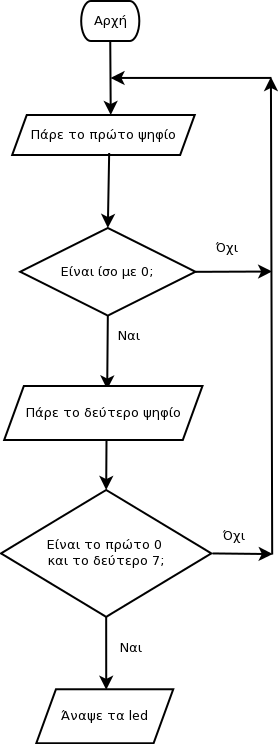
\includegraphics[height=0.5\textheight]{files/flowchart.png}
	\caption{Διάγραμμα ροής}
\end{figure}

\noindent Κυρίως κώδικας:
\inputminted[linenos,obeytabs,fontsize=\footnotesize]{c}{files/part3.S}

\section{}
Σε αυτή την άσκηση ζητείται να απεικονίσουμε στην lcd οθόνη που συνδέουμε στον
AVR αρχικά το μήνυμα TEAM07 (ο αριθμός της ομάδας μας) και στη συνέχεια να
απεικονίζεται το πλήκτρο που πατήθηκε τελευταίο στο keypad 4x4. Επίσης ο
κέρσορας δεν πρέπει να είναι ορατός. Για το σκοπό αυτό, αρχικοποιούμε την
οθόνη, διαβάζουμε το πληκτρολόγιο και περνάμε εντολές  και δεδομένα στην οθόνη
με τις κατάλληλες ρουτίνες που δίνονται έτοιμες στο pdf. Επίσης, σετάρουμε για
είσοδο απ' το keypad την PORTC και για έξοδο στην οθόνη την PORTD. Κάθε φορά
καλούμε την keypad\_rising\_edge αφού έχουμε βάλει στον r24 καθυστερήση 20msec
για τους σπινθηρισμούς, στη συνέχεια φρεσκάρουμε την οθόνη και καλούμε την
lcd\_data για απεικόνιση.  Έπειτα, καθαρίζουμε τη μνήμη ώστε να έχει μόνο το
τελευταίο πλήκτρο που πατήθηκε και διαβάζουμε εκ νέου απ' το πληκτρολόγιο.

\noindent Κυρίως κώδικας:
\inputminted[linenos,obeytabs,fontsize=\footnotesize]{c}{files/part4.S}

\section{}

Σε αυτήν την άσκηση προσομοιώνουμε την λειτουργία ενός συστήματος συναγερμού.
Θέτουμε την θύρα Β ως είσοδο και έπειτα ελέγχουμε συνεχώς αν έχει γίνει
trigger στους αισθητήρες. Άπαξ και έχει γίνει, θέτουμε τον timer για να
αρχίσει να χρονομετρά και καλούμε την συνάρτηση getpass για να διαβάσουμε τον
κωδικό. Ελέγχουμε τα πλήκτρα που εισάγονται με παρόμοιο τρόπο όπως στην άσκηση
3, με την διαφορά ότι άμα έχουμε λάθος πλήκτρο τότε πηγαίνουμε στην ετικέτα
alarm\_on, όπου θέτουμε τον συναγερμό κατά τα ζητούμενα της άσκησης. Σε
περίπτωση που δοθεί ο σωστός κωδικός (τον οποίο έχουμε βάλει κατά σύμβαση
9807) απενεργοποιούμε τον συναγερμό (label alarm\_off), δηλαδή απενεργοποιούμε
τον timer και γραφουμε στην lcd οθόνη alarm off.

\noindent Κυρίως κώδικας:
\inputminted[linenos,obeytabs,fontsize=\footnotesize]{c}{files/part5.S}

\section{}

\noindent Κυρίως κώδικας:
\inputminted[linenos,obeytabs,fontsize=\footnotesize]{c}{files/part6.S}

\end{document}
